\section{Fase di Progettazione}
    \subsection{Struttura del Sito}
    In questa sezione presentiamo una prima bozza grafica delle varie pagine del sito. Ciò ci è servito per avere un'idea generale sull'aspetto che dovrà avere il sito e per avere una base da cui partire per lo sviluppo del layout.
        
    La struttura della gerarchia del sito è suddivisa in pagine, alcune delle quali hanno delle sottopagine:
    \begin{itemize}
        \item Home;
        \item Auto a noleggio;
        \item Auto in vendita;
        \item Contatti;
        \item Pagina di Login;
        \item Pagina di Registrazione;
        \item Area privata (utente generico):
            \begin{itemize}
                \item Area personale;
                \item Dati Personali;
                \item Preventivi;
                \item Noleggi;
                \item Messaggi.
            \end{itemize}
            \item Area privata (utente amministratore):
                \begin{itemize}
                    \item Home amministratore;
                    \item Messaggi;
                    \item Veicoli a noleggio;
                    \item Veicoli in vendita;
                    \item Prenotazione veicoli.
                \end{itemize}
    \end{itemize}

    \subsection{Database}
    Viene riportata la rappresentazione del database, realizzata in fase di progettazione, durante la quale si è discussa la necessità di avere le diverse tabelle e per ogni tabella i necessari attributi, per poi utilizzarli al meglio.
    \begin{figure}[H]
        \centering
        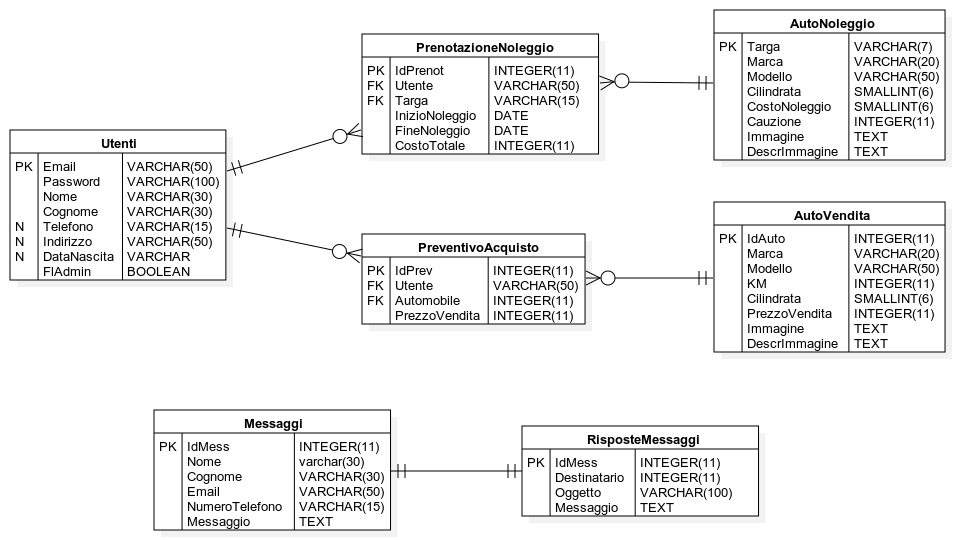
\includegraphics[width=14cm]{./img/database.png}
        \caption{Schema del database}  \label{fig:xray}
    \end{figure}
    Il database è composto dalle seguenti tabelle:
    \begin{itemize}
        \item \textbf{Utenti:} contiene i dati e le credenziali degli utenti registrati, la password è stata codificata con la funzione \textit{password\_hash} di PHP;
        \item \textbf{Messaggi:} contiene i messaggi inviati dagli utenti;
        \item \textbf{AutoVendita:} contiene le auto in vendita;
        \item \textbf{AutoNoleggio:} contiene le auto a noleggio;
        \item \textbf{PreventivoAcquisto:} contiene gli acquisti delle auto effettuati dagli utenti;
        \item \textbf{PrenotazioneNoleggio:} contiene i noleggi delle auto effettuati dagli utenti;
    \end{itemize}

    \subsection{Accessibilità}

\pagebreak